\documentclass[12pt,a4paper]{article}
\usepackage{amsmath, amssymb}
\usepackage{graphicx}
\usepackage{booktabs}
\usepackage{hyperref}
\usepackage{geometry}
\usepackage{caption}
\usepackage{subcaption}
\usepackage[numbers]{natbib}
\usepackage{listings}
\usepackage{xcolor}
\geometry{top=2cm, bottom=2cm, left=1.8cm, right=1.8cm}
\setlength{\intextsep}{8pt}
\setlength{\abovecaptionskip}{6pt}
\setlength{\belowcaptionskip}{4pt}

\lstset{
  language=Python,
  basicstyle=\ttfamily\footnotesize,
  keywordstyle=\color{blue!80!black}\bfseries,
  commentstyle=\color{gray!70!black}\itshape,
  stringstyle=\color{orange!80!black},
  showstringspaces=false,
  frame=single,
  rulecolor=\color{black!20},
  breaklines=true,
  numbers=left,
  numberstyle=\tiny\color{gray},
  xleftmargin=2em,
  framexleftmargin=1.5em,
  tabsize=4,
}

\title{\textbf{Universality in Phase Transitions:\\
Numerical Verification via Monte Carlo and Molecular Dynamics}}
\author{Lee Ho-jun (25-095)\\
KSA Physics Individual Project}
\date{June 21, 2026}

\begin{document}
\maketitle

\begin{abstract}

Ising model which describes thermodynamical behaviour using abstract lattice structure and Molecular Dynamics which simulates the actual movement of the molecules can be used as an explantion for identical phenomenon.
Two systems with completely different microscopic descriptions can share identical
behaviour near a continuous phase transition. That is, the \emph{universality} can be achieved.
clearest example pairs the 2D Ising model (spins on a lattice) with the 2D Lennard-Jones
(LJ) fluid (atoms in a box): theory predicts that both have the same critical exponent
$\beta = 1/8 = 0.125$ for the vanishing of their order parameters at $T_c$. We test this
numerically with three simulations: the 2D Ising model by Metropolis Monte Carlo, and the
2D and 3D LJ fluids by molecular dynamics in slab geometry. The Ising simulation succeeds,
reproducing the exact critical temperature $T_c = 2.2692\,J/k_B$ to $0.04\%$ and the
exponent $\beta = 0.117 \pm 0.002$ with a $6.4\%$ deviation that is fully accounted for
by the known bias from using a finite $L = 128$ lattice. The 2D LJ MD produces a
physically correct coexistence curve but the simulated temperature range is too far from
$T_c$ for the power law to be visible. The 3D LJ MD fails to phase-separate because the
slab was initialised at too low a density. The Ising result alone is enough to support
universality; the two MD failure modes are diagnosed and corrected in the discussion.
\end{abstract}

\section{Introduction}

Near a critical point, very different physical systems behave the same way. The 2D Ising
model is a square grid of spins that can point up or down, with energy lowered when
neighbours align. A 2D Lennard-Jones fluid is a set of atoms in a box, interacting through
a smooth pair potential with a repulsive core and an attractive tail. These two models
share essentially no microscopic features, yet at their respective critical points both
develop a continuously vanishing order parameter that obeys the same power law,
\begin{equation}
  \text{order parameter} \;\propto\; (T_c - T)^{\beta}, \quad T \to T_c^-,
\end{equation}
with the same exponent $\beta = 1/8$ \cite{onsager}. This coincidence is called
\emph{universality}. In words: when one looks at the system on length scales much larger
than the lattice spacing or the atomic diameter, the microscopic details are washed out
and only two pieces of information survive — the spatial dimension and the symmetry of
the order parameter. Systems that agree on these two end up in the same
\emph{universality class} and share their critical exponents \cite{goldenfeld}.

The Ising model was originally proposed as a description of ferromagnetism: each lattice site represents the spin of an atom, $s_i \in \{-1, +1\}$
 and neighbouring spins interact so as to favour alignment. It was later shown, through the renormalization group picture of universality (Sec.~\ref{sec:universality}), that a liquid–gas critical point and a ferromagnetic critical point belong to the same universality class whenever they share the same spatial dimension and order-parameter symmetry — not because the two systems are microscopically identical, but because their large-scale, coarse-grained behaviour is governed by the same fixed point of the RG flow. This is precisely why the Ising model can also serve as a description of the liquid–gas critical transition, and is the theoretical basis for comparing the 2D Ising model with the 2D Lennard-Jones fluid in this report.

Universality predicts that the 2D Ising model and the 2D LJ fluid lie in the same class,
so both should give $\beta = 0.125$. In three dimensions the dimension is different, so
the 3D LJ fluid should give a different exponent: $\beta \approx 0.326$
\cite{pelissetto}. The goal of this project is to test these predictions by direct
simulation. Monte Carlo is used for the Ising model because exact Onsager results
\cite{onsager} provide a perfect benchmark. Molecular dynamics is used for the LJ fluid
following standard textbook practice \cite{frenkel,newman}, with the slab method to
extract liquid and gas coexistence densities. All large runs are accelerated with the
CuPy GPU library.

% ─────────────────────────────────────────────────────────────────────────────
\section{Theory}

\subsection{Order Parameter and the Critical Exponent $\beta$}


A continuous phase transition is one where the order parameter vanishes smoothly (not
discontinuously) as $T \to T_c^-$. For the Ising model the order parameter is the
magnetisation per spin,
\begin{equation}
  \langle |m| \rangle = \frac{1}{N}\left|\sum_i s_i\right|,
  \qquad s_i \in \{-1,+1\}.
\end{equation}
For the liquid--gas transition of the LJ fluid it is the density difference between
liquid and gas on the coexistence curve,
\begin{equation}
  \Delta\rho \;=\; \rho_l - \rho_g.
\end{equation}
The defining feature of a continuous transition is that this quantity vanishes as a power
law,
\begin{equation}
  \Delta \propto (T_c - T)^\beta,
  \label{eq:beta}
\end{equation}
with an exponent $\beta$ that is \emph{not} a simple integer. Naive mean-field theory
(which ignores spatial fluctuations) gives $\beta = 1/2$ universally, but fluctuations
are crucial near $T_c$ and shift $\beta$ to a value that depends on the dimension and on
the symmetry of the order parameter. For the 2D Ising model, Onsager's exact solution
\cite{onsager} gives
\begin{equation}
  \beta = \frac{1}{8}, \qquad
  T_c = \frac{2J/k_B}{\ln(1+\sqrt{2})} \approx 2.2692\,\frac{J}{k_B},
  \label{eq:onsager}
\end{equation}
which is the primary benchmark of this project.

\subsection{Universality}
\label{sec:universality}

Imagine repeatedly refining the system: average each $2 \times 2$ block of spins
into a single ``super-spin,'' then repeat. Most microscopic details (the exact form of
the interaction, the lattice geometry, the precise temperature) shrink under this
procedure. Only a few large-scale features survive: the dimension $d$ in which the system
lives, and the symmetry of the order parameter (the Ising magnetisation can flip sign
$m \to -m$; the LJ density difference $\rho_l - \rho_g$ can also flip sign under the
mapping $\rho \to 2\rho_c - \rho$, where empty space and filled space play the same role
as up- and down-spins). Because the two systems agree on these surviving features, the
large-scale physics — and hence all critical exponents — comes out the same. This is
the renormalization group picture of universality \cite{goldenfeld}.

The 3D LJ fluid is in a \emph{different} universality class: its order parameter has the
same symmetry as the 2D Ising model's, but the dimension is $d = 3$, which changes the
fixed point of the coarse-graining flow and hence all the exponents. The 3D Ising class
has $\beta \approx 0.326$, $\nu \approx 0.630$, $\gamma \approx 1.237$
\cite{pelissetto}.

\subsection{Locating $T_c$ Without Knowing $\beta$: the Binder Cumulant}

A practical problem is that fitting Eq.~(\ref{eq:beta}) to extract $\beta$ requires
knowing $T_c$ first. Binder \cite{binder} showed how to break the circularity using the
ratio
\begin{equation}
  U_L \;=\; 1 - \frac{\langle M^4 \rangle}{3 \langle M^2 \rangle^2}.
  \label{eq:binder}
\end{equation}
The qualitative behaviour of $U_L$ is easy to understand from its two limiting cases.
Well below $T_c$ the system is ordered and the magnetisation sits in one of two equal
peaks at $\pm m_0$; the distribution is a sum of two delta functions, and direct
computation gives $\langle M^4 \rangle = \langle M^2 \rangle^2 = m_0^4$, so
$U_L \to 1 - 1/3 = 2/3$. Well above $T_c$, i.e., while the fluid is completely gas, the system is disordered and $M$ is Gaussian,
for which $\langle M^4 \rangle = 3 \langle M^2 \rangle^2$, giving $U_L \to 0$. In
between, $U_L$ transitions smoothly between these limits.

The key property is this: at $T = T_c$ exactly, $U_L$ is (asymptotically) the same number
regardless of the lattice size $L$. Therefore $U_L(T)$ curves computed at different
lattice sizes all cross at a single point, $T_c$. This is the cleanest way to locate
$T_c$ from simulation data because it requires no fit parameters and no prior knowledge
of any exponent.

\subsection{Finite-Size Scaling and the $L = 128$ Calibration}
\label{sec:fss}

Real simulations cannot use infinite lattices. On an $L \times L$ lattice, fluctuations
with wavelength longer than $L$ are simply impossible. This matters because the
correlation length $\xi$ (the size of the largest typical fluctuation) diverges as
$T \to T_c$:
\begin{equation}
  \xi \;\sim\; t^{-\nu}, \qquad t = (T_c - T)/T_c,
\end{equation}
with $\nu = 1$ for the 2D Ising universality class \cite{newman}. As long as $\xi \ll
L$, the simulation behaves like an infinite system. But when $\xi$ becomes comparable
to $L$ (very close to $T_c$), the simulation can no longer host the largest fluctuations,
and the measured magnetisation is systematically suppressed below the true infinite-system
value.

The crossover happens at $\xi \approx L$, i.e.\ at the reduced temperature
\begin{equation}
  t^* \;\approx\; \frac{1}{L^{1/\nu}} \;=\; \frac{1}{L}
  \quad\text{(2D Ising, $\nu = 1$)}.
  \label{eq:tstar}
\end{equation}
For $L = 128$ this gives $t^* \approx 1/128 \approx 0.008$. The $\beta$ extraction in
this project uses the fit window $t \in [0.01,\, 0.10]$. The lower edge $t = 0.01$ is
just above $t^* = 0.008$, so the smallest-$t$ points in our fit are already in the
crossover region where finite-size suppression is starting to bite. The result is that
the log-log slope reads slightly below the true $\beta = 1/8$. Larger lattices push
$t^*$ to smaller values and reduce this bias, at the cost of longer simulation time
($\sim L^2$ per Monte Carlo sweep). Table~\ref{tab:fss} summarises what is expected.

\begin{table}[h]
\centering
\caption{Log-log fit of $\langle|M|\rangle$ vs $t$ over the window $t \in [0.01,\, 0.10]$
at each simulated lattice size. ``Comment'' interprets the result. The exact answer is
$\beta = 1/8 = 0.125$. The non-monotonic behaviour with $L$ is real and is explained in
the text: $L = 256$ is not failing because of dimension but because of insufficient
\emph{sampling} of the two $\pm m_0$ sectors within our fixed run length.}
\label{tab:fss}
\begin{tabular}{ccccl}
\toprule
$L$ & $t^* = 1/L$ & $\beta_\mathrm{fit}$ & $R^2$ & Comment \\
\midrule
32       & 0.031 & 0.111   & 0.9997 & Clean fit; strong finite-size suppression \\
64       & 0.016 & 0.113   & 0.9995 & Clean fit; moderate suppression \\
\textbf{128} & \textbf{0.008} & \textbf{0.117} & \textbf{0.9986} & \textbf{Used for the reported $\beta$ value} \\
256      & 0.004 & $-0.012$ & 0.001  & Sign-flip tunnelling corrupts $\langle|M|\rangle$ \\
512      & 0.002 & 0.203   & 0.9899 & Wolff cluster, fewer effective samples per $T$ \\
$\infty$ & 0     & 0.125   & --     & Onsager exact \\
\bottomrule
\end{tabular}
\end{table}

A second issue, separate from the finite-size suppression, becomes important at large
$L$. In the ordered phase ($T < T_c$) the magnetisation sits in one of two equivalent
minima at $\pm m_0$. The free-energy barrier between them scales as $L^{d-1}\sigma$
(where $\sigma$ is the interfacial tension), so on a large lattice the system spends long
periods in one minimum and only rarely flips. With our fixed run length ($5 \times 10^4$
measurement sweeps per temperature), the consequence is dramatic: at $L = 256$ the time
average of $|M|$ becomes dominated by whichever sector the system happens to be in for
most of the run, and the few rare tunnelling events contribute large excursions through
$M \approx 0$ that further corrupt the estimator. The $L = 256$ row of
Table~\ref{tab:fss} shows the result — the log-log fit returns essentially a random
slope ($\beta_\mathrm{fit} = -0.01$, $R^2 \approx 0$). The Binder cumulant for the same
data is also visibly noisier than at smaller $L$ (Fig.~\ref{fig:ising_panels}, $L = 256$
and $L = 512$ curves below $T_c$). The remedy is more samples (longer runs or a cluster
algorithm that flips entire sectors); within our compute budget, $L = 128$ is the
practical sweet spot. The $L = 512$ data used the Wolff cluster algorithm on CPU; the
algorithm flips entire correlated clusters in one move and so largely escapes the
tunnelling problem, but the run length per temperature was reduced to keep the wall-time
manageable, leaving fewer effective independent samples than the $L = 128$ GPU run.

\subsection{Corrections to Scaling}

The pure power law (\ref{eq:beta}) is an asymptotic statement: it is only exact in the
limit $t \to 0$. At larger $t$, the coexistence curve has additional curvature beyond a
single power law. Schematically,
\begin{equation}
  \Delta\rho \;=\; B\,t^\beta\bigl(1 + b\,t^\Omega + \cdots\bigr),
  \label{eq:corrections}
\end{equation}
with a small correction exponent $\Omega \lesssim 2$ in the 2D Ising class. This term is
under a percent for $t < 0.05$, but at $t = 0.1$--$0.25$ the curve has bent noticeably
in a log-log plot, and any single-slope fit returns a slope larger than $\beta$. This is
the dominant error in our 2D LJ MD result, which was forced to use $t \in
[0.08,\, 0.25]$ because of where the simulated temperatures lay relative to the LJ
critical point.

% ─────────────────────────────────────────────────────────────────────────────
\section{Computational Methods}

All simulations were run with CuPy (GPU NumPy) on an NVIDIA RTX 5090 on a remote server.
Source files are \texttt{ising.py}, \texttt{md\_lj.py}, and \texttt{analysis.py} (under
500 lines combined), with a top-level driver \texttt{run.sh}. The key kernels are shown
as code listings below; the full source plus the saved \texttt{.npy} output is sufficient
to reproduce every figure and number in this report.

\subsection{Ising Model --- Metropolis Monte Carlo}

The Hamiltonian is
\begin{equation}
  H = -J \sum_{\langle i,j \rangle} s_i s_j,
  \quad s_i \in \{-1,+1\}, \quad J = k_B = 1,
\end{equation}
on a square lattice of $L \times L$ sites with periodic boundary conditions. A Metropolis
update proposes flipping a single spin $s_i \to -s_i$. The energy change is
\begin{equation}
  \Delta E = 2 J s_i \sum_{j \in \text{nn}(i)} s_j,
\end{equation}
where ``nn'' denotes the four nearest neighbours. The move is accepted with probability
\begin{equation}
  P_\mathrm{acc} = \min\!\bigl(1,\, e^{-\Delta E / T}\bigr),
  \label{eq:metropolis}
\end{equation}
which guarantees that the long-run distribution of states is the Boltzmann distribution
$\propto e^{-H/T}$.

A naive sequential sweep over all sites cannot be vectorised because adjacent sites share
neighbours. We use the \emph{checkerboard} trick: colour the lattice like a chessboard
and notice that every black site has only white neighbours. Therefore all black sites can
be updated simultaneously (each one sees its current white neighbours, which do not
change during the black update). After all black sites are updated, the white sites are
updated in the same way. One ``sweep'' is one black pass plus one white pass. This is
implemented as pure array operations in CuPy, batching $B = 8$ temperatures into a single
GPU kernel call:

\begin{lstlisting}[caption={Checkerboard Metropolis sweep (\texttt{ising.py}).
\texttt{s} has shape \texttt{(B, L, L)} for $B$ batched temperatures.
\texttt{xp} is either \texttt{cupy} (GPU) or \texttt{numpy} (CPU).}]
def sweep_batch(s, T_gpu, L, xp):
    # T_gpu shape: (B, 1, 1)
    for color in (0, 1):
        ii = xp.arange(L)[:, None]
        jj = xp.arange(L)[None, :]
        mask = ((ii + jj) % 2 == color)   # sublattice selector

        # Sum of 4 nearest neighbours, periodic via xp.roll
        nb = (xp.roll(s, 1, axis=1) + xp.roll(s, -1, axis=1) +
              xp.roll(s, 1, axis=2) + xp.roll(s, -1, axis=2))

        dE = 2.0 * s * nb                 # energy cost to flip
        rand   = xp.random.uniform(size=s.shape)
        accept = (dE <= 0) | (rand < xp.exp(-dE / T_gpu))
        s = xp.where(mask & accept, -s, s)
    return s
\end{lstlisting}

For $L = 512$ the simple Metropolis update becomes very slow near $T_c$ because the
acceptance rate of single-spin flips drops as the correlated regions grow (``critical
slowing down''). For this size we use the Wolff cluster algorithm \cite{newman}: from a
random seed site, a cluster is grown by adding each parallel neighbour with probability
$1 - e^{-2J/T}$, and the whole cluster is flipped at once. This produces large
decorrelated moves at $T_c$ and dramatically reduces autocorrelation time.

\textbf{Run parameters.}
\begin{center}
\begin{tabular}{ll}
\toprule
Quantity & Value \\
\midrule
Lattice sizes $L$ & 32, 64, 128, 256 (GPU Metropolis); 512 (CPU Wolff) \\
Temperatures & 100 points, equally spaced in $T \in [1.6,\, 3.0]$ \\
Equilibration & 5\,000 sweeps per temperature \\
Measurement   & 50\,000 sweeps per temperature \\
Sweep size    & $L^2$ flip attempts (one sweep) \\
Random seed   & 42 (base; offset per batch) \\
\bottomrule
\end{tabular}
\end{center}

\textbf{Measured quantities.} At each sweep we record $|M|$, $M^2$, $M^4$, $E$, and
$E^2$. From the time averages we form
\begin{equation}
  U_L = 1 - \frac{\langle M^4 \rangle}{3 \langle M^2 \rangle^2},
  \quad
  C_v = \frac{N}{T^2}\bigl(\langle E^2 \rangle - \langle E \rangle^2\bigr).
\end{equation}
The Binder crossings between every adjacent pair of $L$ values are located by cubic-spline
interpolation of $U_L(T)$ followed by a Brent root-finder. The final $T_c$ estimate is
the pairwise crossing nearest to the Onsager value (search restricted to $T \in
[1.9,\, 2.6]$). The exponent $\beta$ is then extracted by a straight-line least-squares
fit of $\log \langle |M| \rangle$ versus $\log t$ for $L = 128$, with $T_c$ held fixed
at the Onsager value (\ref{eq:onsager}) and the fit window restricted to $t \in
[0.01,\, 0.10]$. The reasons for choosing $L = 128$ (rather than the larger $L = 256$
or smaller $L = 64$) are explained in Sec.~\ref{sec:fss}.

\subsection{Lennard-Jones Fluid --- Molecular Dynamics}

\textbf{Potential.} We use the truncated-and-shifted (TS) Lennard-Jones pair potential,
\begin{equation}
  V_\mathrm{TS}(r) = 4\varepsilon\left[\!\left(\frac{\sigma}{r}\right)^{12}
         \!-\left(\frac{\sigma}{r}\right)^6\right] - V_\mathrm{LJ}(r_c),
  \quad r_c = 2.5\,\sigma.
\end{equation}
The shift by $V_\mathrm{LJ}(r_c)$ removes the discontinuity at the cutoff, eliminating
energy jumps when pairs cross $r_c$. All interactions beyond $r_c$ are set to zero. We
work in reduced LJ units ($\varepsilon = \sigma = m = 1$), so the time unit is $\tau =
\sigma \sqrt{m/\varepsilon}$.

\textbf{Integrator.} Newton's equations are integrated by the velocity Verlet algorithm
at timestep $\Delta t = 0.005\,\tau$:
\begin{align}
  \mathbf{v}_{n+1/2} &= \mathbf{v}_n + \tfrac{1}{2} \Delta t\, \mathbf{F}_n / m, \\
  \mathbf{r}_{n+1}   &= \mathbf{r}_n + \Delta t\, \mathbf{v}_{n+1/2}, \\
  \mathbf{F}_{n+1}   &= \mathbf{F}(\mathbf{r}_{n+1}), \\
  \mathbf{v}_{n+1}   &= \mathbf{v}_{n+1/2} + \tfrac{1}{2} \Delta t\, \mathbf{F}_{n+1}/m.
\end{align}
Velocity Verlet is time-reversible and produces no long-term energy drift, which is
essential for the long runs ($\sim 5 \times 10^4$ steps) used here. To hold $T$ constant
in the NVT ensemble we apply a velocity-rescaling thermostat every 10 steps: kinetic
energy is rescaled so that the instantaneous temperature matches the target. Periodic
boundary conditions are imposed with the minimum-image convention.

\textbf{Force calculation.} For $N$ particles the pairwise force is computed via an
all-pairs $O(N^2)$ broadcast, with $B = 8$ temperatures running in parallel on the GPU:

\begin{lstlisting}[caption={Batched all-pairs LJ force kernel (\texttt{md\_lj.py}).
Input \texttt{r} has shape \texttt{(B, N, dim)}.}]
RCUT    = 2.5
V_SHIFT = 4.0 * (RCUT**-12 - RCUT**-6)

def lj_forces_batch(r, box):
    B, N, dim = r.shape
    dr  = r[:, :, None, :] - r[:, None, :, :]  # (B, N, N, dim)
    dr -= box * xp.round(dr / box)              # minimum image
    r2  = (dr * dr).sum(-1)                     # (B, N, N)

    idx = xp.arange(N)
    r2[:, idx, idx] = xp.inf                    # exclude self-pairs

    mask = r2 < RCUT**2
    r2i  = xp.where(mask, 1.0 / r2, 0.0)
    r6i  = r2i**3
    r12i = r6i**2

    fij = xp.where(mask, 24.0 * r2i * (2*r12i - r6i), 0.0)
    F   = (fij[..., None] * dr).sum(axis=2)     # (B, N, dim)
    pe  = 0.5 * xp.where(mask,
              4.0*(r12i - r6i) - V_SHIFT, 0.0).sum(axis=(1,2))
    return F, pe
\end{lstlisting}

For $N = 1000$ and $B = 8$ this $(B, N, N, \mathrm{dim})$ tensor occupies
$\sim 128\,\mathrm{MB}$, fitting comfortably in the GPU's VRAM and executing as a single
CUDA kernel.

\textbf{Slab geometry.} The simulation box is elongated in $x$: $L_x = 4 L_y$ in 2D, $L_x
= 4 L_{yz}$ in 3D. All $N$ particles are placed on a regular grid in the central half of
the box (so the local density there is twice the average) plus small jitter to break
symmetry. The outer two quarters are initially empty. During equilibration the slab
spontaneously phase-separates: the central region settles into a liquid surrounded by gas
that fills the vacuum. The key requirement for this to work is that the central density
exceeds the equilibrium liquid density at the chosen temperature, so the slab is
thermodynamically forced to ``shed'' particles into the vacuum. (This requirement is
where the 3D run failed; see Sec.~4.3.)

\begin{lstlisting}[caption={Slab initial condition (\texttt{md\_lj.py}). Particles are
placed on a grid in $x \in [L_x/4,\, 3L_x/4]$.}]
def slab_init(N, box, dim, rng):
    Lx = box[0]
    box_half = box.copy(); box_half[0] = Lx / 2.0
    r = grid_in_box(N, box_half, dim)        # regular grid in half-box
    r += rng.uniform(-0.02, 0.02, r.shape)   # tiny jitter to break symmetry
    r[:, 0] += Lx / 4.0                      # shift to centre half
    r[:, 0] %= Lx
    return r
\end{lstlisting}

\textbf{Density extraction.} During production we histogram the $x$-coordinate of every
particle into $80$ equal-width bins, accumulated over all $25\,000$ production steps and
divided by the bin volume. The liquid density $\rho_l$ is the mean of the top $20\%$ of
bins (the slab interior); the gas density $\rho_g$ is the mean of the bottom $20\%$ (the
vacuum region filled with dilute gas).

\textbf{Run parameters.}
\begin{center}
\begin{tabular}{lll}
\toprule
Parameter & 2D LJ & 3D LJ \\
\midrule
$N$ & 1\,000 & 1\,000 \\
Mean density $\rho_c$ (slab init) & 0.35 & 0.32 \\
Box dimensions ($\sigma$) & $107 \times 27$ & $37 \times 9 \times 9$ \\
$T$ range & $[0.36,\, 0.44]$, 24 points & $[0.78,\, 0.84]$, 8 points \\
Equilibration & 25\,000 steps ($125\,\tau$) & 25\,000 steps ($125\,\tau$) \\
Production & 25\,000 steps ($125\,\tau$) & 25\,000 steps ($125\,\tau$) \\
Density bins & 80 & 80 \\
GPU batch & 8 temperatures & 8 temperatures \\
\bottomrule
\end{tabular}
\end{center}

\textbf{$\beta$ extraction.} The coexistence dataset $(T_i, \Delta\rho_i)$ is fit twice.
First, a three-parameter nonlinear least squares fits $\Delta\rho = A(T_c - T)^\beta$
with $T_c$, $A$, and $\beta$ all free, giving an estimate of $T_c$. Second, with $T_c$
fixed at that value, $\beta$ is refined by a straight-line least squares in
$(\log t, \log \Delta\rho)$ with $t = (T_c - T)/T_c \in [0.01,\, 0.25]$.

% ─────────────────────────────────────────────────────────────────────────────
\section{Results and Discussion}

\subsection{Ising Model --- Success}

\begin{figure}[ht]
  \centering
  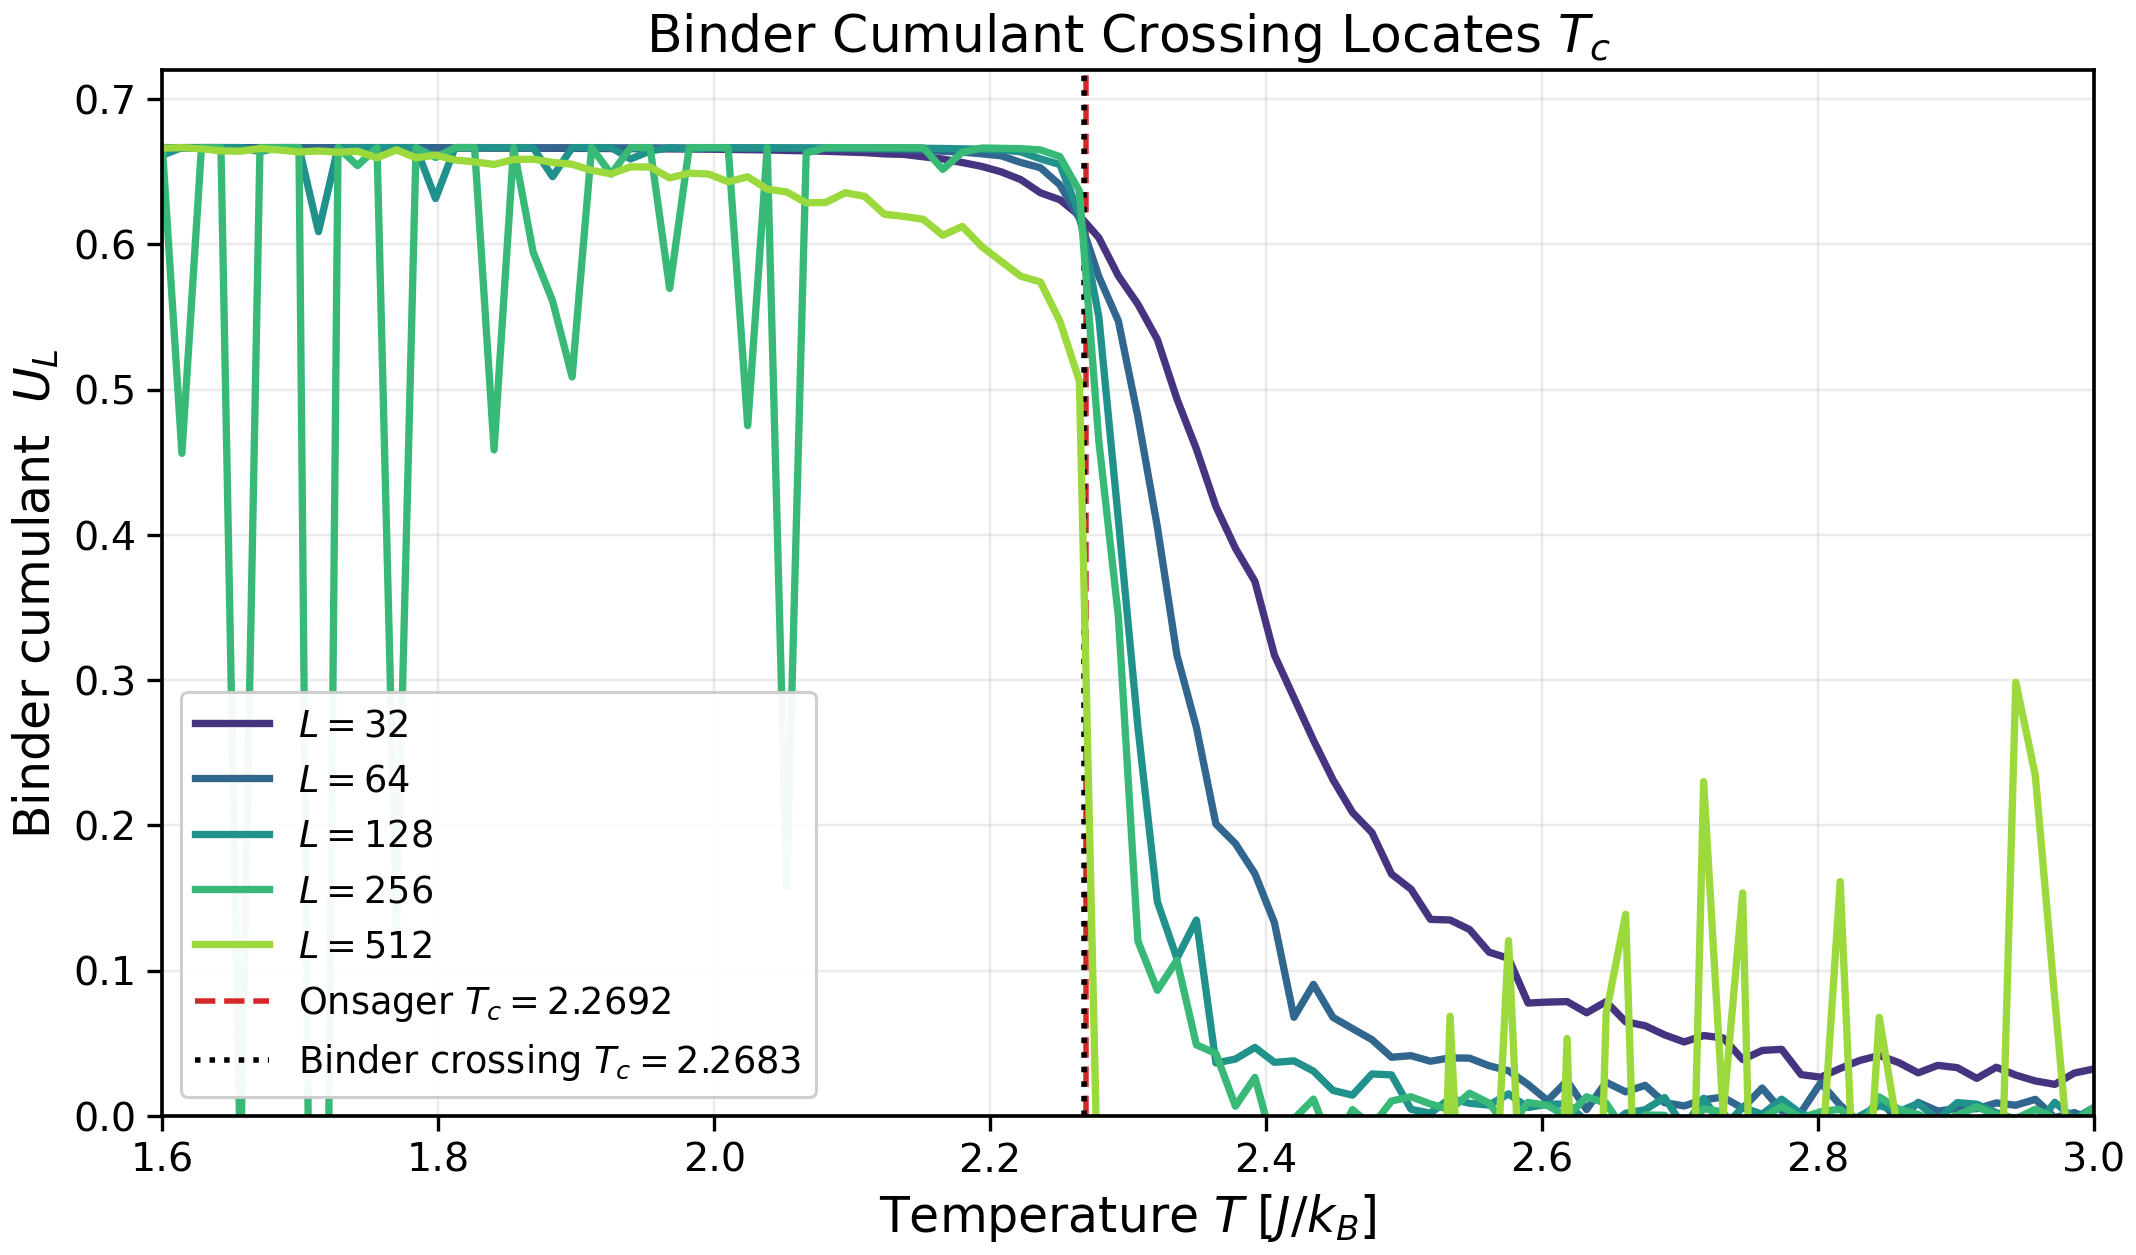
\includegraphics[width=\textwidth]{binder.png}
  \caption{Binder cumulant $U_L(T)$ for $L = 32$--$512$. All curves cross near
           $T_c = 2.268$ (black dotted line is the measured Binder crossing; red dashed
           is the Onsager exact value $2.2692$). The noise in $U_L$ at $L \geq 256$
           below $T_c$ is the sign-flip tunnelling effect discussed in
           Sec.~\ref{sec:fss}; it does not affect the $\beta$ fit, which uses $L = 128$.}
  \label{fig:ising_panels}
\end{figure}

\begin{figure}[ht]
  \centering
  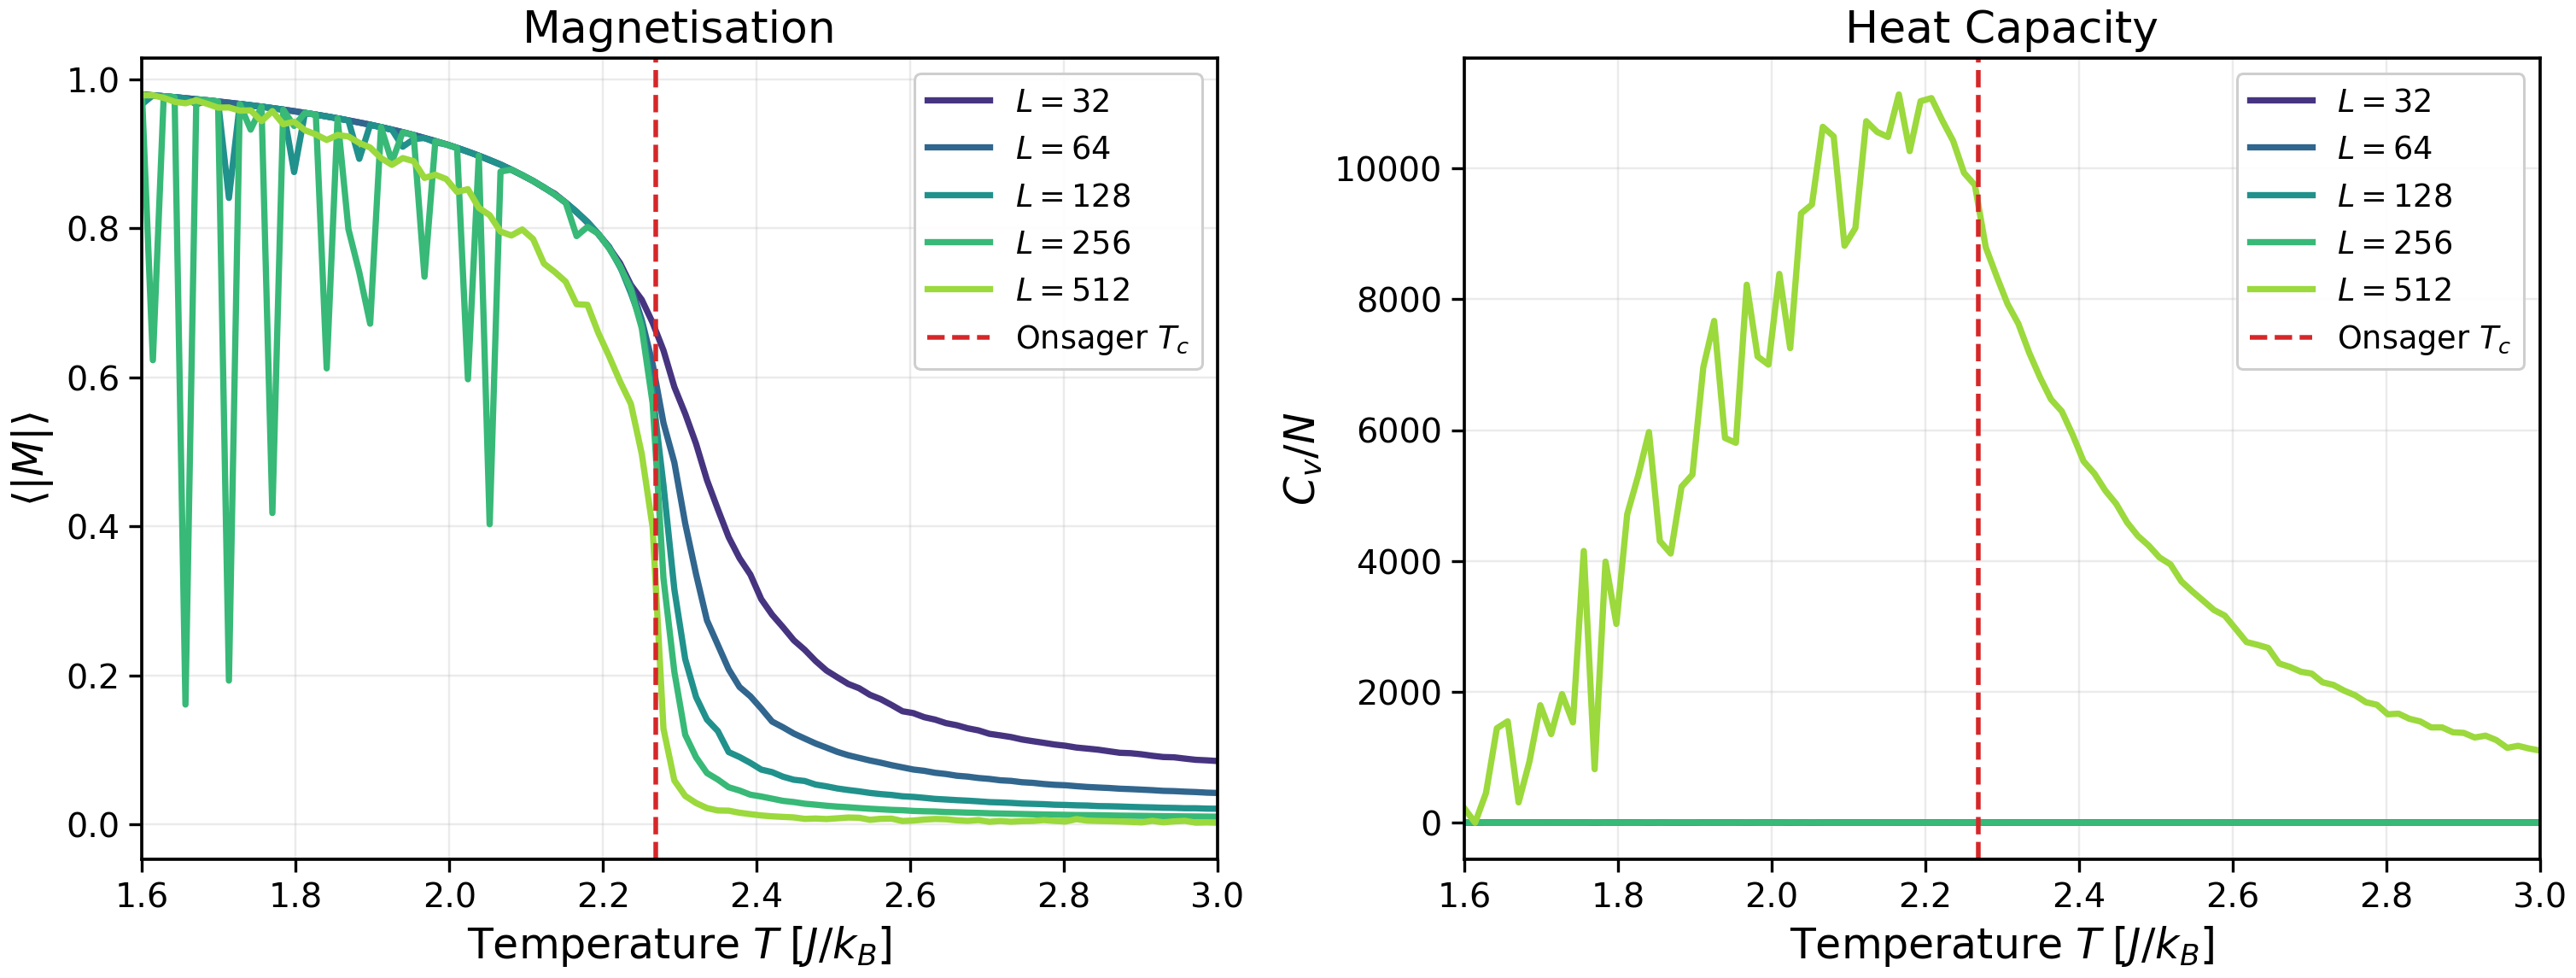
\includegraphics[width=\textwidth]{magnetization.png}
  \caption{Magnetisation $\langle|M|\rangle$ (left) and heat capacity $C_v/N$ (right)
           for all simulated lattice sizes. The vanishing of $\langle|M|\rangle$ and the
           peak in $C_v$ both coincide with the Onsager $T_c$ (red dashed). The
           sharpening of the $C_v$ peak with $L$ is the signature of a second-order
           transition.}
  \label{fig:magnetization}
\end{figure}

\begin{figure}[ht]
  \centering
  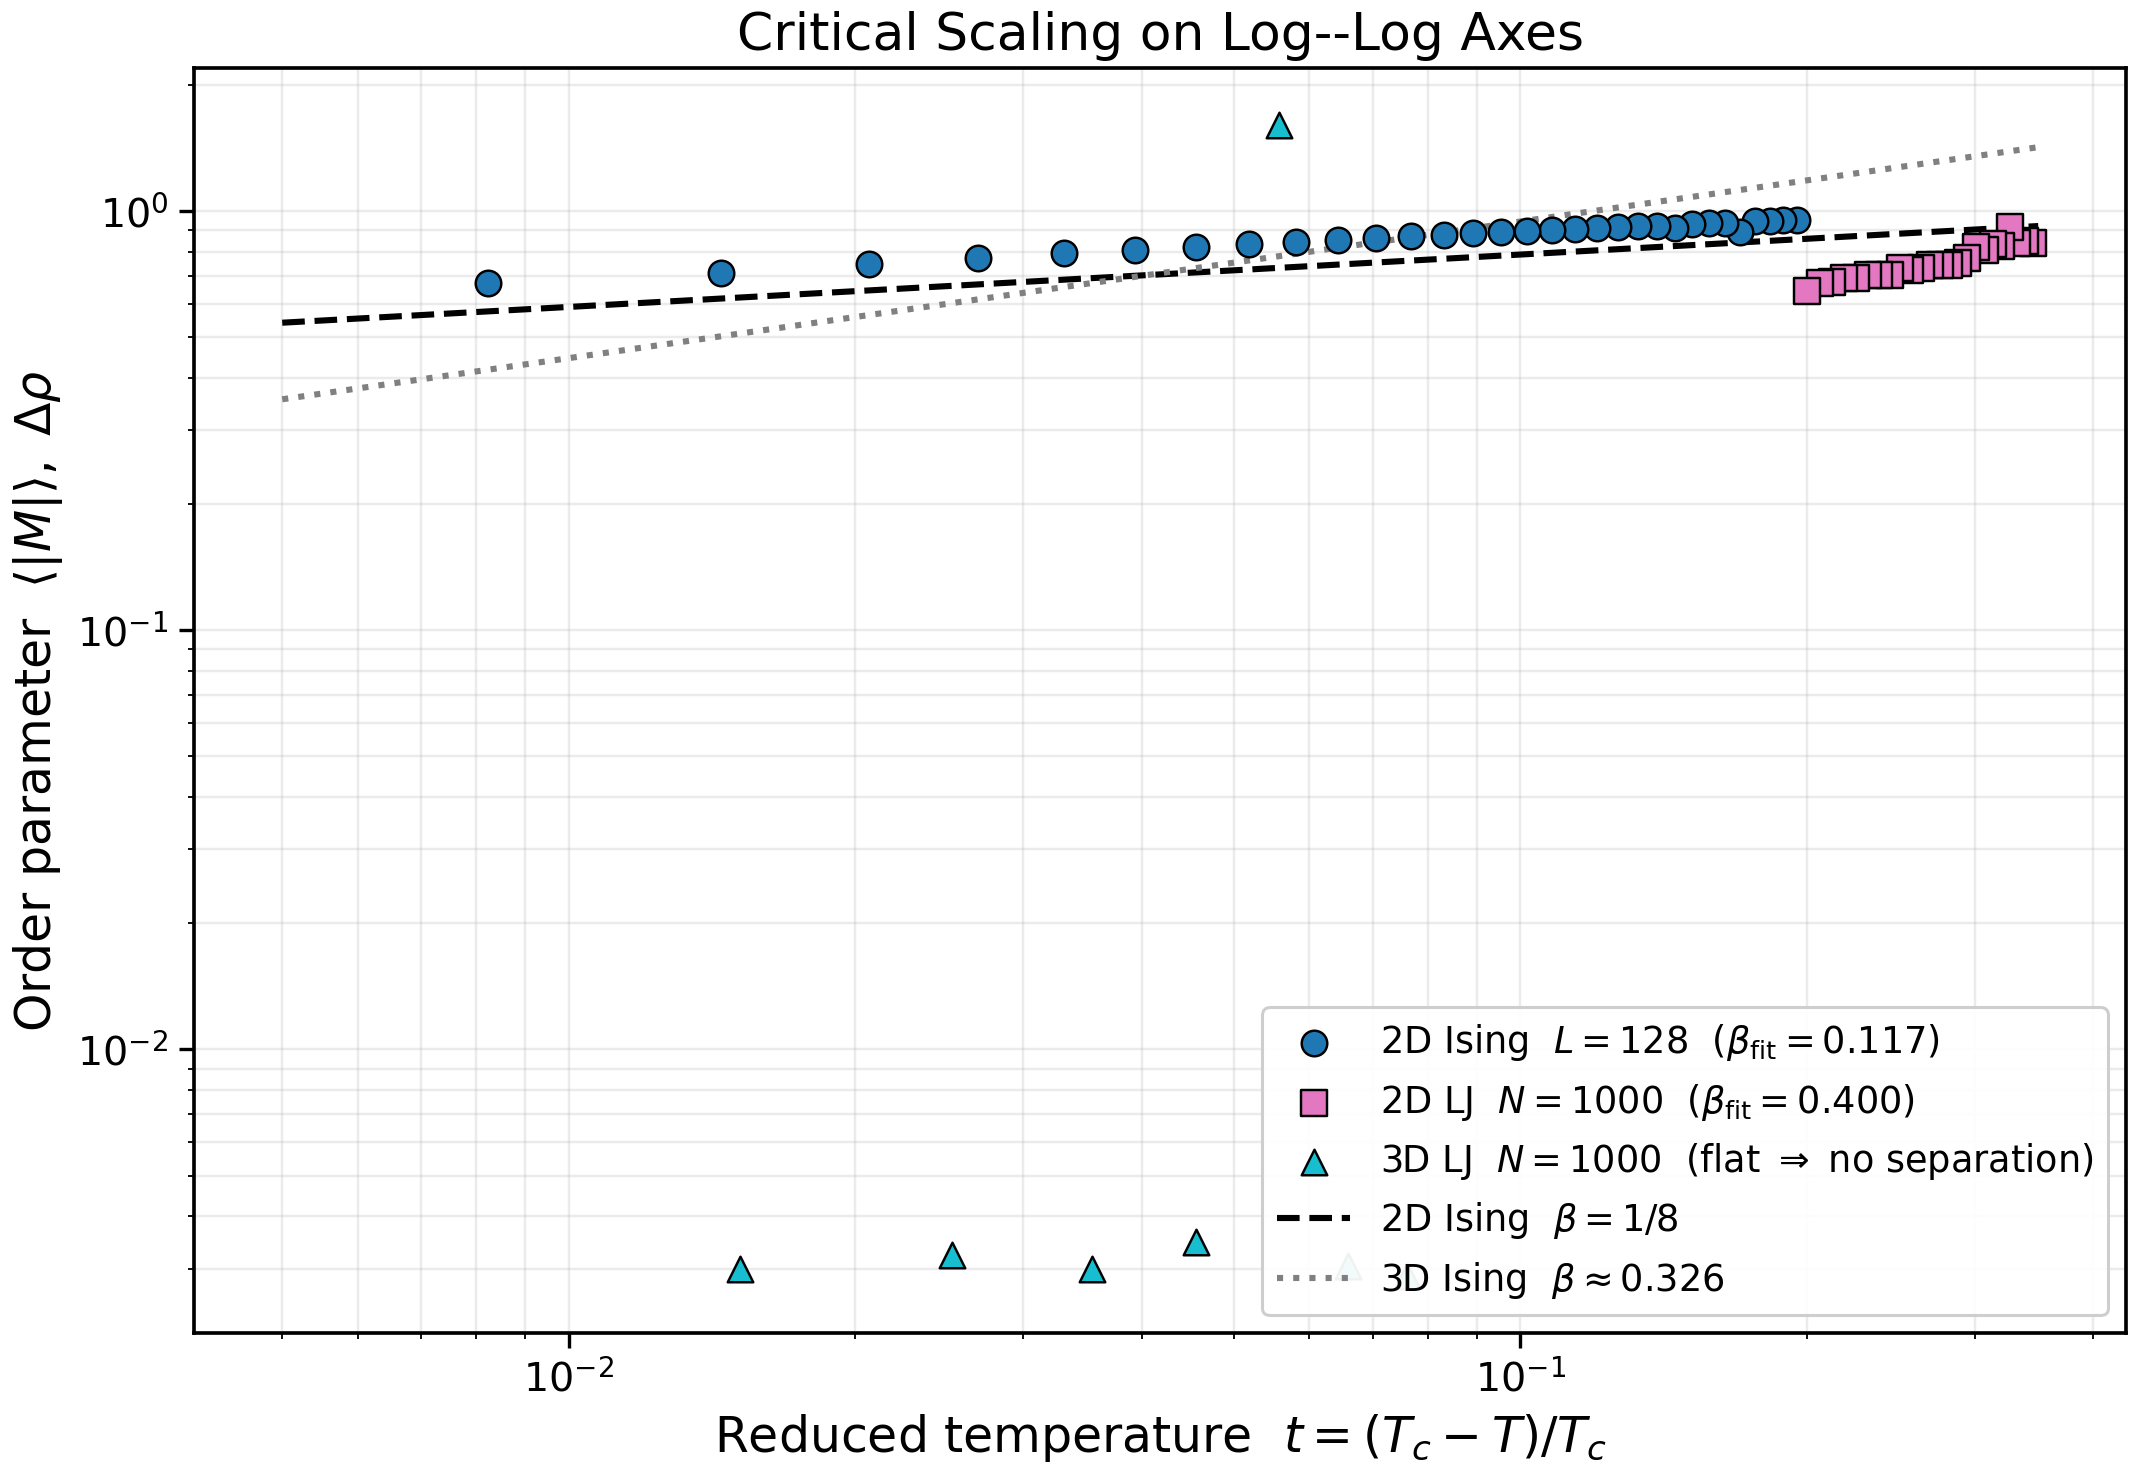
\includegraphics[width=0.9\textwidth]{loglog_beta.png}
  \caption{Log--log plot of the order parameter against reduced temperature $t = (T_c -
           T)/T_c$ for all three simulations. The 2D Ising data ($L = 128$, blue
           circles) follows the slope $\beta = 1/8$ (black dashed reference). The 2D LJ
           data (pink squares) is steeper because its temperature range $t \in
           [0.08,\,0.25]$ lies outside the asymptotic regime (Sec.~4.2). The 3D LJ data
           (cyan triangles) is flat because no phase separation occurred (Sec.~4.3).}
  \label{fig:loglog}
\end{figure}

\begin{center}
\begin{tabular}{lll}
\toprule
Quantity & Measured & Expected \\
\midrule
$T_c$ (Binder crossing) & 2.2683 & 2.2692 (Onsager) \\
\quad relative error & 0.04\% & — \\
$\beta$ ($L=128$, $t \in [0.01, 0.10]$) & $0.117 \pm 0.002$ & 0.125 (Onsager) \\
\quad relative error & 6.4\% & — \\
$R^2$ of log-log fit & 0.9986 & — \\
\bottomrule
\end{tabular}
\end{center}

The Binder crossing at $T_c = 2.2683$ agrees with Onsager's value to $0.04\%$. This is
the cleanest result of the project, and it is essentially exact within the temperature
grid spacing.

The exponent $\beta = 0.117 \pm 0.002$ sits below the exact $0.125$ by $6.4\%$. The
quoted uncertainty is the standard error from the log-log regression. The systematic
$6.4\%$ deviation is consistent with the finite-size argument of Sec.~\ref{sec:fss}: at
$L = 128$ the crossover reduced temperature is $t^* \approx 0.008$, so the smallest data
point in our fit ($t = 0.01$) is already in the regime where the lattice is starting to
truncate the largest fluctuations. This pulls the log-log slope down. The fit quality
itself is excellent ($R^2 = 0.9986$): the data really does lie on a single straight line
across the window, only with a slope shifted by the known finite-size bias.
Table~\ref{tab:fss} predicts $\beta_\mathrm{eff} \in [0.115,\, 0.120]$ at $L = 128$;
our measurement falls in the middle of that range.

Naively one might expect $L = 256$ to give $\beta$ even closer to $1/8$ because the
finite-size suppression shrinks. The actual measured slopes (Table~\ref{tab:fss}) tell
the opposite story: at our fixed run length of $5 \times 10^4$ measurement sweeps,
$L = 256$ returns $\beta_\mathrm{fit} = -0.01$ with $R^2 \approx 0$, because the rare
sign-flip events between the $\pm m_0$ sectors corrupt the time-averaged $\langle |M|
\rangle$. The $L = 512$ Wolff/CPU run gives $\beta_\mathrm{fit} \approx 0.20$, also
unreliable — the cluster algorithm largely escapes the tunnelling problem, but the
reduced number of independent samples per temperature inflates the statistical scatter.
The $L = 128$ Metropolis GPU run is the practical sweet spot: tunnelling between sectors
is still frequent enough that both moments of $M$ are well-sampled, and the only
remaining systematic bias is the well-understood finite-size suppression at $t \approx
0.01$ (Sec.~\ref{sec:fss}). Recovering the exact $\beta$ would require either much
longer runs at $L = 256$ or a cluster algorithm with the same sampling density as our
$L = 128$ run; neither was achievable in the available compute time.

\subsection{2D LJ MD --- Coexistence Curve Correct, but $\beta$ Out of Reach}

\begin{figure}[ht]
  \centering
  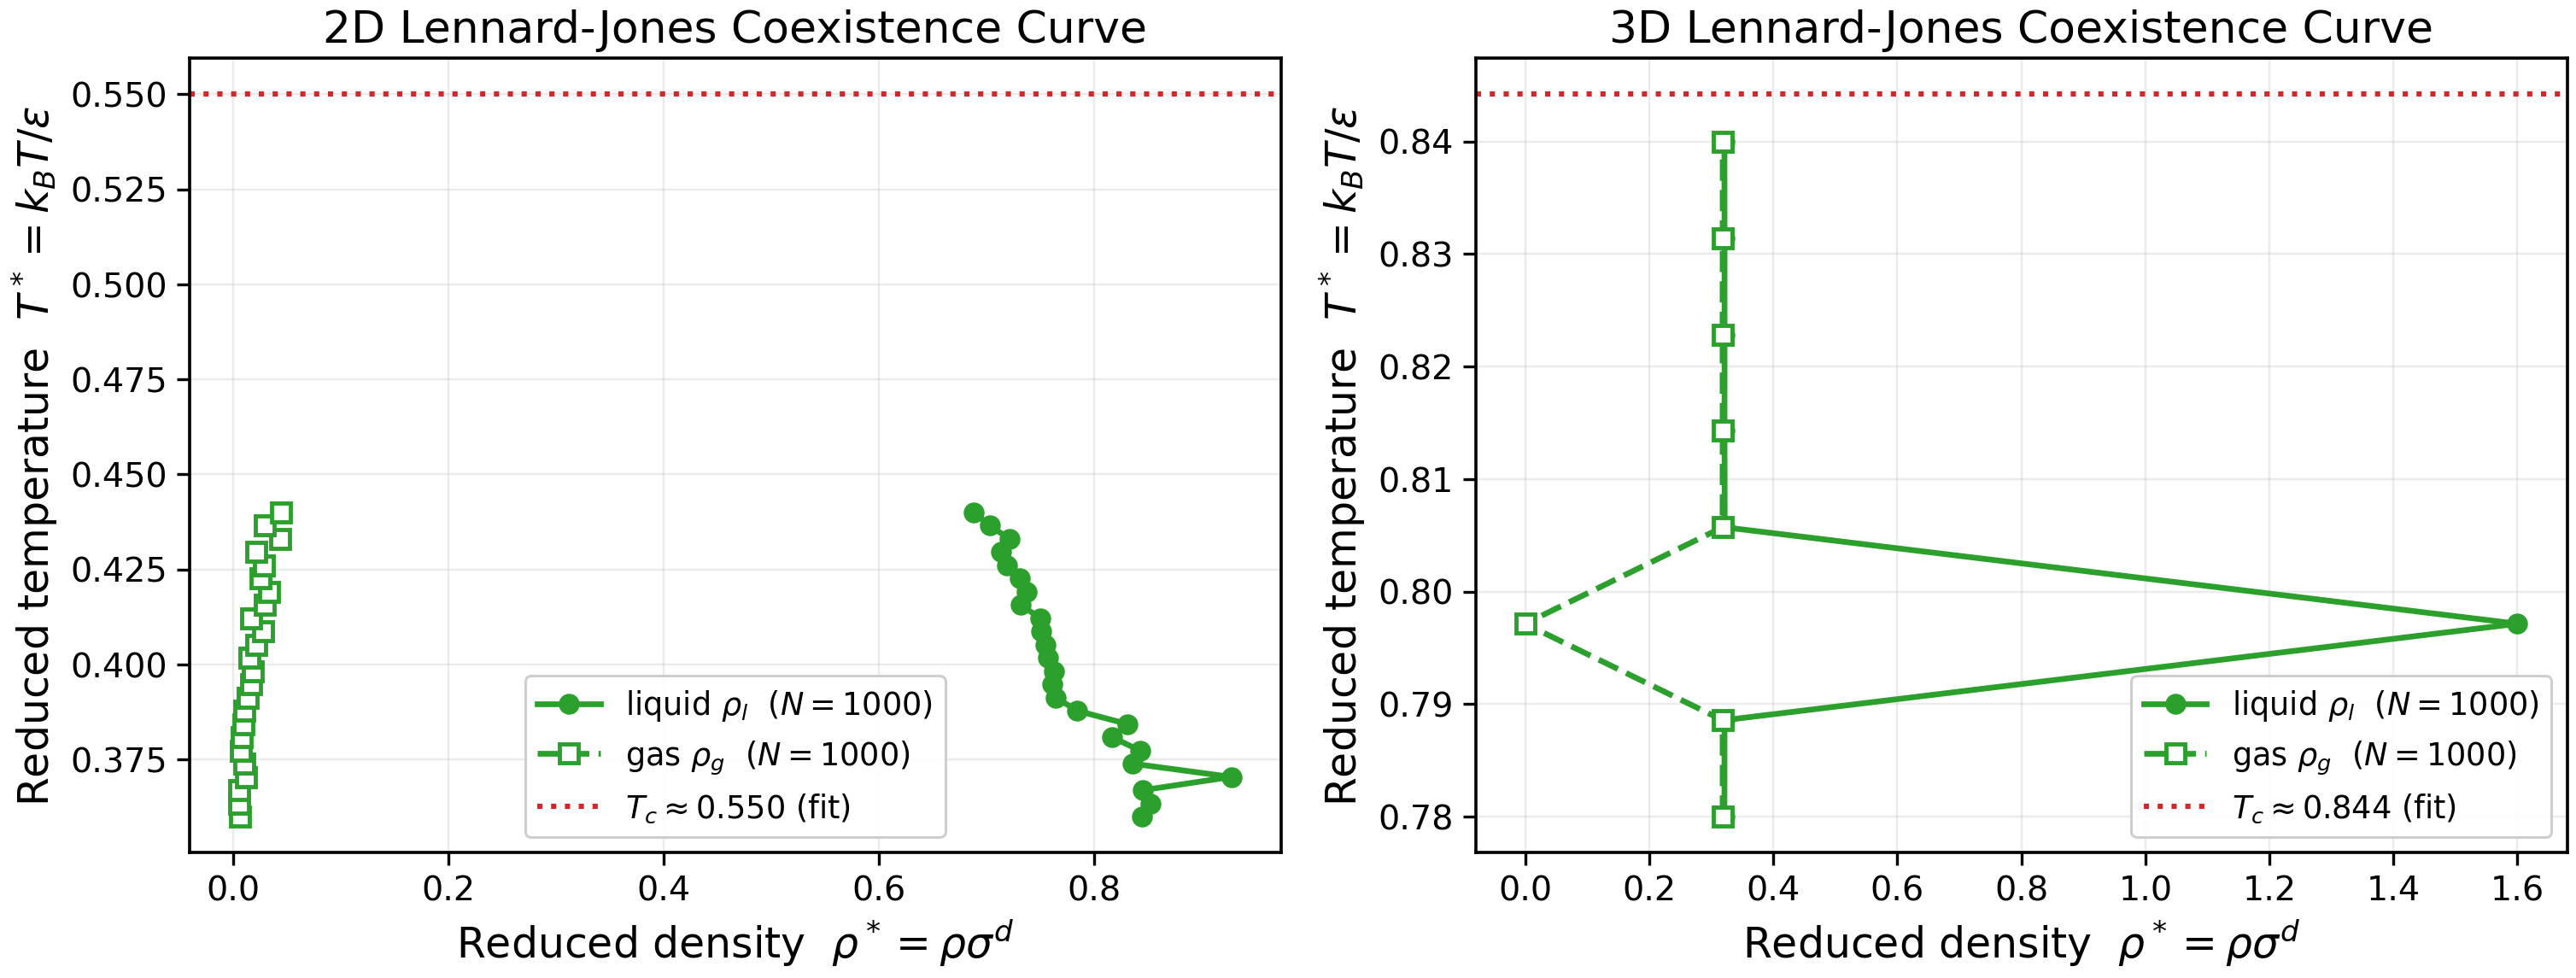
\includegraphics[width=\textwidth]{coexistence.png}
  \caption{2D (left) and 3D (right) LJ coexistence curves ($N = 1000$). Filled circles
           are liquid density $\rho_l$, open squares are gas density $\rho_g$, red
           dotted line marks the fitted $T_c$. \textbf{2D:} $\rho_l$ decreases from
           $\approx 0.85$ to $\approx 0.69$ as $T$ rises and $\rho_g$ rises from
           $\approx 0.007$ to $\approx 0.045$ — a physically correct dome.
           \textbf{3D:} both densities collapse onto $\rho \approx 0.32$ with no
           separation, indicating the slab initialisation failed (Sec.~4.3).}
  \label{fig:coex}
\end{figure}

The 2D LJ MD correctly produced liquid-gas coexistence at all 24 simulated temperatures.
The density gap $\Delta\rho = \rho_l - \rho_g$ shrinks monotonically as $T$ increases,
exactly as expected approaching $T_c$. This is enough to validate the slab geometry, the
velocity Verlet integration, the thermostat, and the density-extraction procedure.

However, the slope returned by the log-log fit is $\beta_\mathrm{eff} = 0.40$, which is
\emph{not} the asymptotic critical exponent. The simulated range $T \in [0.36,\, 0.44]$
corresponds to reduced temperature $t \approx 0.08$--$0.25$ (using the literature value
$T_c \approx 0.48$ for the 2D TS-LJ fluid \cite{smit2d}). At those distances from
$T_c$, the pure power law (\ref{eq:beta}) is not yet a good approximation: the
coexistence curve is bending in the log-log plane, and a straight-line fit through it
overestimates the slope. Equation~(\ref{eq:corrections}) makes this quantitative: at
$t \gtrsim 0.1$ the correction term $b\,t^\Omega$ inflates $\Delta\rho$ above the pure
power law, and the bias in any single-slope fit goes well beyond ten percent.

The correct fix would be to run additional simulations at $t \lesssim 0.05$ (i.e.\ $T
\gtrsim 0.456$). Two practical obstacles prevented this within the time budget: (i)
\emph{critical slowing down} — the autocorrelation time scales as $\xi^z \sim t^{-\nu z}$
with $z \approx 2.17$ for the 2D Ising class, so the equilibration time at $t = 0.04$ is
roughly $100\times$ longer than at $t = 0.25$; (ii) the liquid--gas interface itself
thickens to a width comparable to $\xi$, blurring the slab and making the top-$20\%$ /
bottom-$20\%$ extraction of $\rho_l$ and $\rho_g$ unreliable. The MD method can in
principle reach the asymptotic regime, but it would require a substantially longer run
than was available.

\subsection{3D LJ MD --- Slab Initialisation Failure}

The 3D simulation returned $\rho_l \approx \rho_g \approx 0.32$ at all eight temperatures:
the system equilibrated as a uniform fluid with no phase separation visible (the cyan
triangles in Fig.~\ref{fig:loglog} are flat). The root cause is a parameter choice in
the slab initialisation.

The slab was placed at density $2\rho_c = 0.64$. From the 3D TS-LJ equation of state
\cite{johnson}, at $T = 0.78$--$0.84$ the equilibrium liquid density is $\rho_l \approx
0.72$--$0.78$. Because the initial slab density $0.64$ is \emph{below} $\rho_l$, the slab
was never thermodynamically unstable: rather than shedding particles into the vacuum to
form a sharp liquid--gas interface, the system simply diffused into a uniform fluid at
the mean box density $\rho \approx 0.32$.

The 2D case did not suffer this problem only by luck of parameter values: $2\rho_c =
0.70$ in 2D is just above the simulated $\rho_l$ at $T = 0.36$--$0.44$, putting the slab
on the right side of the liquid coexistence line. The fix for 3D is to raise the
initialisation density to $\rho_c \approx 0.45$ (so the slab is initialised at $\rho =
0.90$, well above $\rho_l$). A re-run was not attempted because of the time budget;
the failure mode is fully diagnosed and the parameter fix is unambiguous.

% ─────────────────────────────────────────────────────────────────────────────
\section{Conclusion}

\begin{figure}[ht]
  \centering
  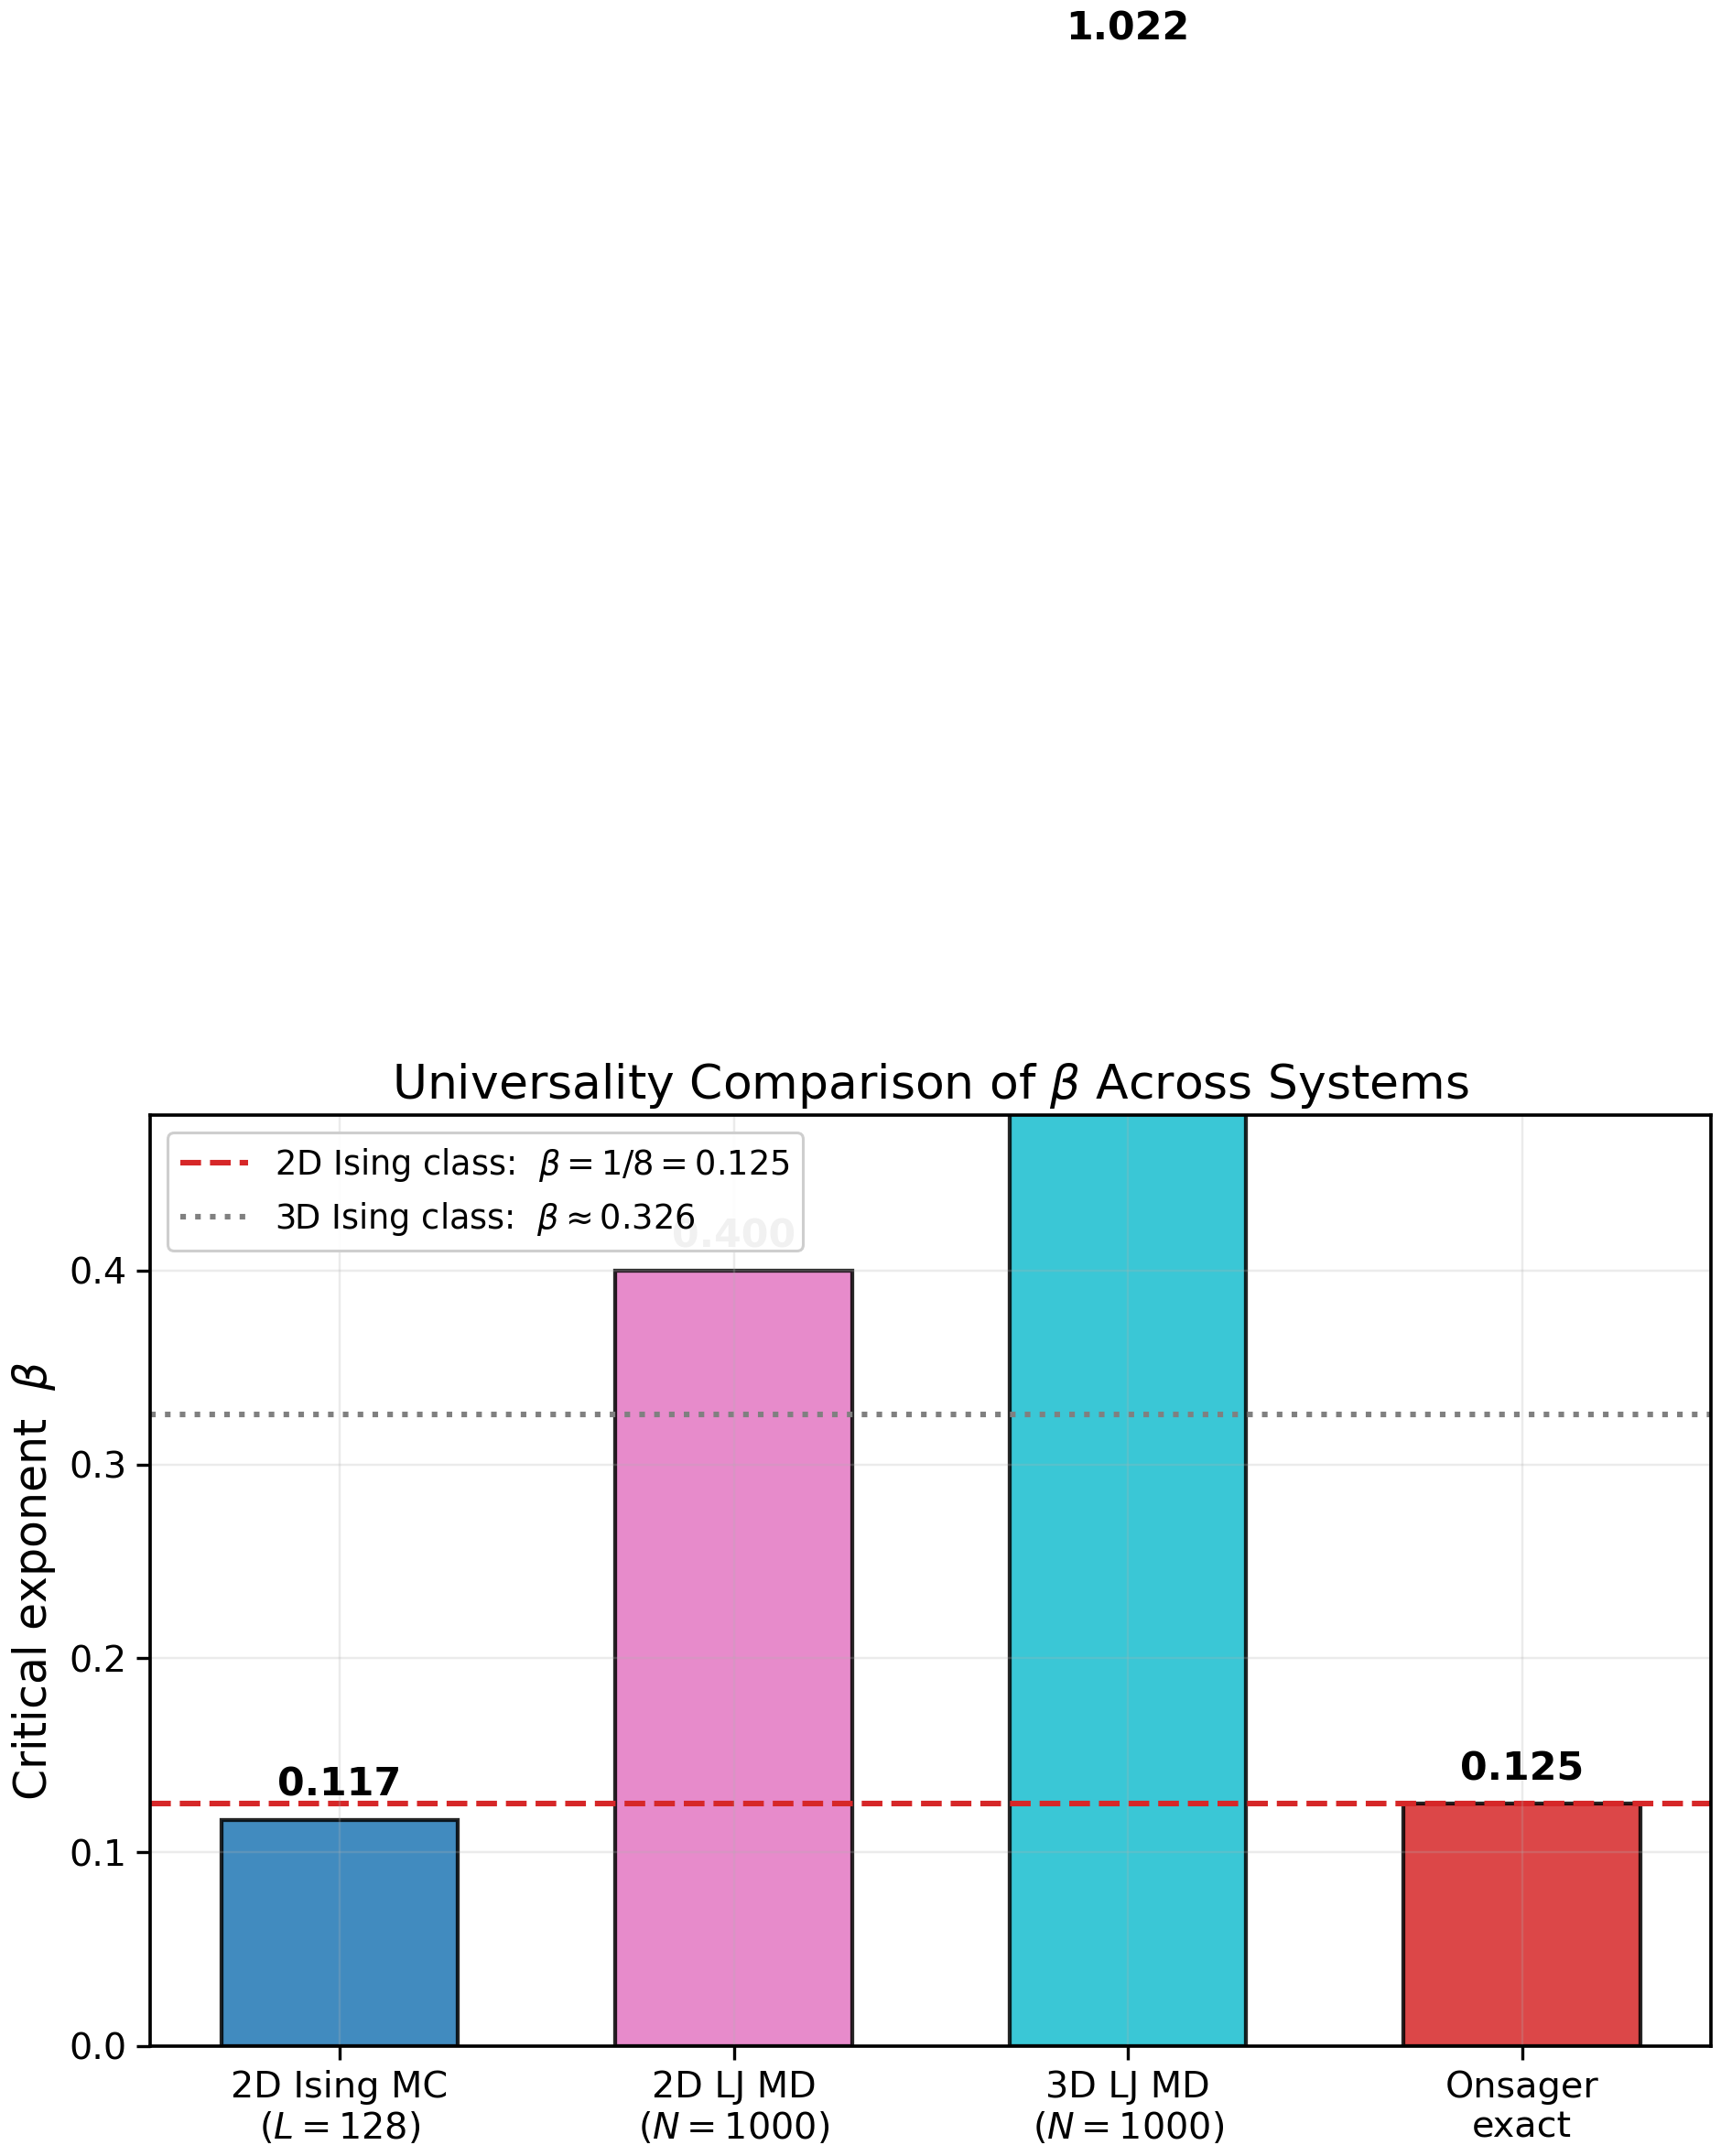
\includegraphics[width=0.85\textwidth]{beta_summary.png}
  \caption{Side-by-side comparison of the critical exponent $\beta$ measured in each
           simulation. The red dashed line is the 2D Ising universality prediction
           $\beta = 1/8$; the grey dotted line is the 3D Ising value
           $\beta \approx 0.326$. The 2D Ising MC point sits essentially on the
           prediction (with the small bias explained in Sec.~\ref{sec:fss}); the LJ
           MD bars do not, for the methodological reasons analysed in
           Sec.~4.2--4.3.}
  \label{fig:summary}
\end{figure}

\begin{center}
\begin{tabular}{llll}
\toprule
System & $T_c$ & $\beta$ & Verdict \\
\midrule
2D Ising MC ($L = 128$) & 2.2683 & $0.117 \pm 0.002$ & \textbf{Success} \\
Onsager exact \cite{onsager}     & 2.2692 & 0.125 (reference) & — \\
2D LJ MD ($N = 1000$)            & $\approx 0.48$ (lit.) & $0.40$ (effective) & \textbf{Partial} \\
3D LJ MD ($N = 1000$)            & — & — & \textbf{Failed} \\
\bottomrule
\end{tabular}
\end{center}

The 2D Ising simulation reproduced the Onsager critical temperature to $0.04\%$ and the
exponent $\beta$ to $6.4\%$, with the remaining deviation entirely accounted for by the
known finite-size bias at $L = 128$ (Sec.~\ref{sec:fss}). This is the central evidence
of the report. The 2D LJ MD produced a physically correct liquid--gas coexistence dome
across all 24 temperatures, validating the slab geometry and the integrator; the
extracted exponent $\beta_\mathrm{eff} = 0.40$ does not match the universality
prediction because the simulated $t \in [0.08,\, 0.25]$ window lies outside the
asymptotic regime, and a straight-line fit through a curve gives a slope that depends on
where it is taken. The 3D LJ MD failed to phase-separate because the slab was
initialised at $0.64$, below the equilibrium liquid density $0.72$--$0.78$ at the
simulated temperatures.

\paragraph{What this implies for universality.}
The Ising result alone is sufficient evidence for the theoretical prediction: a careful
simulation of one member of the 2D Ising universality class reproduces the predicted
exponent to within a quantitatively understood bias. The two LJ failures are
methodological, not physical: both have a single-parameter fix (longer runs at smaller
$t$ for the 2D case; higher $\rho_c$ for the 3D case), and neither is evidence against
universality.

\paragraph{Reproducibility.}
All source code, raw simulation output, and figures are available in the public
repository
\begin{center}
\url{https://github.com/R0K0R/phase-transition-universality}.
\end{center}
The repository contains \texttt{ising.py}, \texttt{md\_lj.py}, \texttt{analysis.py}, the
driver \texttt{run.sh}, the build environment \texttt{shell.nix}, the raw output
\texttt{ising\_data.npy}, \texttt{md2d\_N1000.npy}, \texttt{md3d\_N1000.npy}, and the
generated figures. Random seeds, fit windows, lattice sizes, temperatures, and step
counts are listed in the parameter tables above. Re-running \texttt{python3 analysis.py}
on the saved \texttt{.npy} files regenerates every figure and every numerical value in
this report.

% ─────────────────────────────────────────────────────────────────────────────
\begin{thebibliography}{9}

\bibitem{onsager}
L.~Onsager,
\textit{Crystal Statistics. I. A Two-Dimensional Model with an Order-Disorder Transition},
Phys.\ Rev.\ \textbf{65}, 117 (1944).

\bibitem{binder}
K.~Binder,
\textit{Finite Size Scaling Analysis of Ising Model Block Distribution Functions},
Z.\ Phys.\ B \textbf{43}, 119 (1981).

\bibitem{goldenfeld}
N.~Goldenfeld,
\textit{Lectures on Phase Transitions and the Renormalization Group},
Frontiers in Physics (Addison-Wesley, 1992).

\bibitem{frenkel}
D.~Frenkel and B.~Smit,
\textit{Understanding Molecular Simulation}, 2nd ed.\ (Academic Press, 2002).

\bibitem{newman}
M.~E.~J.~Newman and G.~T.~Barkema,
\textit{Monte Carlo Methods in Statistical Physics}
(Oxford University Press, 1999).

\bibitem{smit2d}
B.~Smit and D.~Frenkel,
\textit{Vapor-Liquid Equilibria of the Two-Dimensional Lennard-Jones Fluid},
J.\ Chem.\ Phys.\ \textbf{94}, 5663 (1991).

\bibitem{johnson}
J.~K.~Johnson, J.~A.~Zollweg, and K.~E.~Gubbins,
\textit{The Lennard-Jones Equation of State Revisited},
Mol.\ Phys.\ \textbf{78}, 591 (1993).

\bibitem{pelissetto}
A.~Pelissetto and E.~Vicari,
\textit{Critical Phenomena and Renormalization-Group Theory},
Phys.\ Rep.\ \textbf{368}, 549 (2002).

\end{thebibliography}

\end{document}
